\documentclass{article}
\usepackage[polish]{babel}
\usepackage{lmodern}  
\usepackage{graphicx}
\usepackage{float}
\usepackage{titlesec}
\usepackage{datetime}
\usepackage{geometry}
\usepackage{booktabs}
\usepackage{placeins}
\usepackage{minted}
\usepackage{xcolor}
\usepackage{listings}

\geometry{
 a4paper,
 left=25mm,
 top=25mm,
 }
\newdateformat{daymonthyear}{\THEDAY .\THEMONTH .\THEYEAR}
\title{
  \center
\includegraphics[width=\textwidth]{src/images/logo_PWr_kolor_poziom.png}\\
  \fontsize{28pt}{30pt}\selectfont Sprawozdanie 4\\
  \fontsize{14pt}{30pt}\selectfont }
\author{Krzysztof Zalewa}
\date{\daymonthyear\today}
\renewcommand*\contentsname{Spis treści}
\renewcommand{\tablename}{Tabela}


\begin{document}
  \maketitle
  \pagebreak
  \tableofcontents
  \section{Problem komiwojażera}
  \section{Specyfikacja sprzętu}
  \section{Procedura badawcza}
  \section{Badania}
  \subsection{Algorytm losowy (ang. Random)}
  Lorem
  \subsubsection{Opis algorytmu}
  \subsubsection{Lista kroków}
  \subsubsection{Założenia badawcze}

  \subsubsection{Wyniki}
  \subsubsection{Wnioski}
  \subsection{Algorytm najbliższego sąsiada (ang. Nearest neighbour)}
  Lorem
  \subsubsection{Opis algorytmu}
  \subsubsection{Lista kroków}
  \subsubsection{Założenia badawcze}
  \subsubsection{Wyniki}
  \begin{table}[ht]
\centering
\begin{tabular}{rrrrrrr}
\toprule
 & \multicolumn{3}{c}{Symetryczne} & \multicolumn{3}{c}{Asymetryczne} \\
Rozmiar/Gęstość & 30\% & 60\% & 100\% & 30\% & 60\% & 100\% \\
\midrule
8 & 0.000102 & 0.000119 & 0.000031 & 0.000098 & 0.000079 & 0.000032 \\
9 & 0.000114 & 0.000170 & 0.000046 & 0.000172 & 0.000141 & 0.000045 \\
10 & 0.000339 & 0.000239 & 0.000066 & 0.000341 & 0.000338 & 0.000067 \\
11 & 0.000390 & 0.000386 & 0.000092 & 0.000538 & 0.000321 & 0.000115 \\
12 & 0.000822 & 0.000707 & 0.000122 & 0.000822 & 0.000707 & 0.000123 \\
\bottomrule
\end{tabular}
\caption{Czasy wykonania algorytmu dla macierzy symetrycznych i niesymetrycznych}
\label{tab:mean_time_nearest-neighbourresoult}
\end{table}
\begin{table}[ht]
\centering
\begin{tabular}{rrrrrrr}
\toprule
 & \multicolumn{3}{c}{Symetryczne} & \multicolumn{3}{c}{Asymetryczne} \\
Rozmiar/Gęstość & 30\% & 60\% & 100\% & 30\% & 60\% & 100\% \\
\midrule
8 & 30867 & N/A & 15230 & 38267 & N/A & 24012 \\
9 & N/A & 34161 & 9417 & N/A & 17918 & 17589 \\
10 & N/A & 39705 & 18569 & N/A & N/A & 19255 \\
11 & N/A & 33758 & 19573 & N/A & 19994 & 17246 \\
12 & N/A & N/A & 17710 & N/A & 15781 & 16216 \\
\bottomrule
\end{tabular}
\caption{Wyniki algorytmu dla macierzy symetrycznych i niesymetrycznych}
\label{tab:resoult_nearest-neighbourresoult}
\end{table}
\begin{table}[ht]
\centering
\begin{tabular}{rrrrrrr}
\toprule
 & \multicolumn{3}{c}{Symetryczne} & \multicolumn{3}{c}{Asymetryczne} \\
Rozmiar/Gęstość & 30\% & 60\% & 100\% & 30\% & 60\% & 100\% \\
\midrule
8 & 0.000000 & N/A & 0.190000 & 0.330000 & N/A & 0.160000 \\
9 & N/A & 0.200000 & 0.320000 & N/A & 0.170000 & 0.000000 \\
10 & N/A & 0.010000 & 0.130000 & N/A & N/A & 0.300000 \\
11 & N/A & 0.050000 & 0.250000 & N/A & 0.020000 & 0.260000 \\
12 & N/A & N/A & 0.040000 & N/A & 0.000000 & 0.310000 \\
\bottomrule
\end{tabular}
\caption{Błędy w wynikach algorytmu dla macierzy symetrycznych i niesymetrycznych}
\label{tab:error_nearest-neighbourresoult}
\end{table}

  \FloatBarrier

  \begin{figure}[ht]
    \centering
    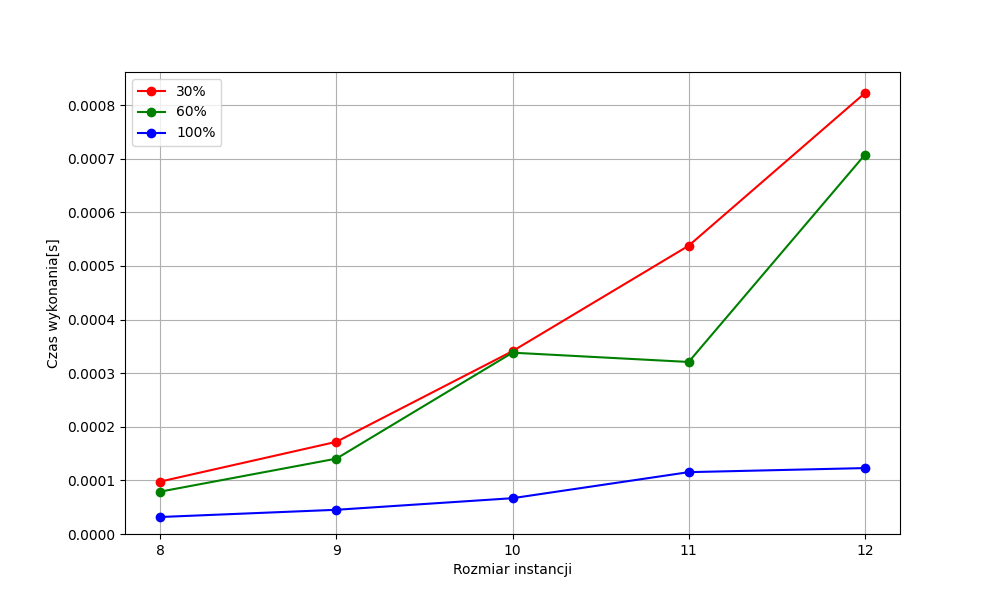
\includegraphics[width=\textwidth]{src/plots/asymnearest-neighbourresoult.png}
    \caption{Wyniki dla macierzy symetrycznych o różnych gęstościach}
    \label{fig:asm_nn}
  \end{figure}
  \begin{figure}[ht]
    \centering
    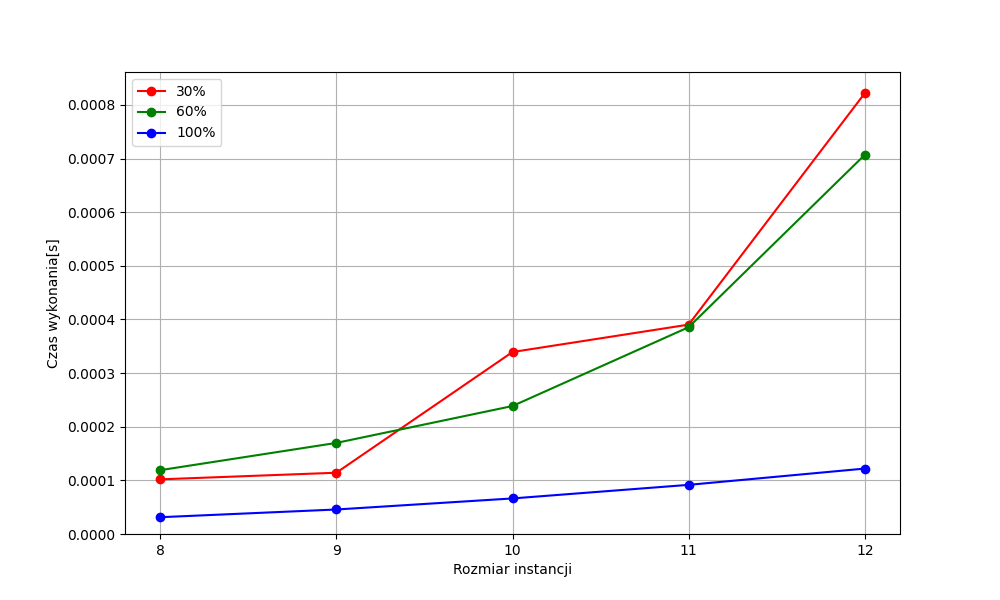
\includegraphics[width=\textwidth]{src/plots/symnearest-neighbourresoult.png}
    \caption{Wyniki dla macierzy symetrycznych o różnych gęstościach}
    \label{fig:sm_nn}
  \end{figure}
  \FloatBarrier
  \subsubsection{Wnioski}

  \subsection{Algorytm siłowy (ang. Brute-force)}
  Lorem
  \subsubsection{Opis algorytmu}
  \subsubsection{Lista kroków}
  \subsubsection{Założenia badawcze}
  \subsubsection{Wyniki}
  \begin{table}[ht]
\centering
\begin{tabular}{rrrrrrr}
\toprule
 & \multicolumn{3}{c}{Symetryczne} & \multicolumn{3}{c}{Asymetryczne} \\
Rozmiar/Gęstość & 30\% & 60\% & 100\% & 30\% & 60\% & 100\% \\
\midrule
8 & 0.000584 & 0.001455 & 0.002964 & 0.000594 & 0.005930 & 0.006764 \\
9 & 0.022613 & 0.012452 & 0.000671 & 0.007114 & 0.047743 & 0.002322 \\
10 & 0.125065 & 0.106813 & 0.049782 & 0.383290 & 0.478340 & 0.565129 \\
11 & 0.658866 & 1.088163 & 2.050599 & 4.200745 & 5.931383 & 0.191078 \\
12 & 2.315414 & 5.455512 & 4.550668 & 50.459794 & 63.293619 & 25.105833 \\
\bottomrule
\end{tabular}
\caption{Czasy wykonania algorytmu dla macierzy symetrycznych i niesymetrycznych}
\label{tab:mean_time_brute-forceresoult}
\end{table}
\begin{table}[ht]
\centering
\begin{tabular}{rrrrrrr}
\toprule
 & \multicolumn{3}{c}{Symetryczne} & \multicolumn{3}{c}{Asymetryczne} \\
Rozmiar/Gęstość & 30\% & 60\% & 100\% & 30\% & 60\% & 100\% \\
\midrule
8 & 30867 & 22264 & 12806 & 28719 & 16035 & 18843 \\
9 & 23923 & 28513 & 7129 & 26942 & 13728 & 17589 \\
10 & 24562 & 39212 & 16436 & 26726 & 14207 & 14841 \\
11 & 40077 & 32101 & 15619 & 35236 & 19117 & 13657 \\
12 & 39712 & 26906 & 17016 & 31919 & 13727 & 12343 \\
\bottomrule
\end{tabular}
\caption{Wyniki algorytmu dla macierzy symetrycznych i niesymetrycznych}
\label{tab:resoult_brute-forceresoult}
\end{table}
\begin{table}[ht]
\centering
\begin{tabular}{rrrrrrr}
\toprule
 & \multicolumn{3}{c}{Symetryczne} & \multicolumn{3}{c}{Asymetryczne} \\
Rozmiar/Gęstość & 30\% & 60\% & 100\% & 30\% & 60\% & 100\% \\
\midrule
8 & 0.000000 & 0.000000 & 0.000000 & 0.000000 & 0.020000 & 0.090000 \\
9 & 0.000000 & 0.000000 & 0.000000 & 0.000000 & 0.100000 & 0.000000 \\
10 & 0.000000 & 0.000000 & 0.000000 & 0.090000 & 0.150000 & 0.000000 \\
11 & 0.000000 & 0.000000 & 0.000000 & 0.110000 & 0.060000 & 0.000000 \\
12 & 0.000000 & 0.000000 & 0.000000 & 0.030000 & 0.130000 & 0.000000 \\
\bottomrule
\end{tabular}
\caption{Błędy w wynikach algorytmu dla macierzy symetrycznych i niesymetrycznych}
\label{tab:error_brute-forceresoult}
\end{table}

  \FloatBarrier

  \begin{figure}[ht]
    \centering
    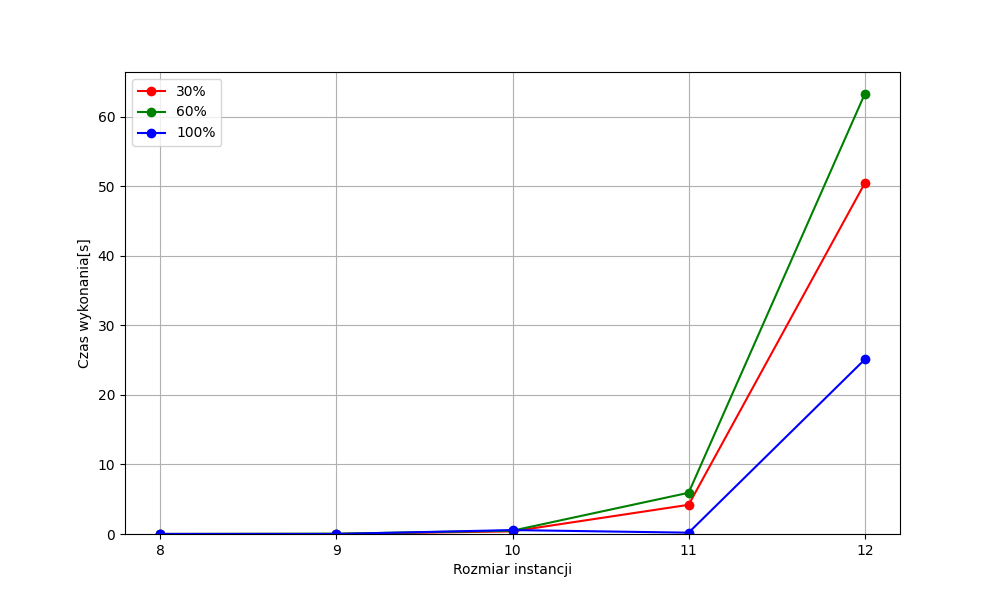
\includegraphics[width=\textwidth]{src/plots/asymbrute-forceresoult.png}
    \caption{Wyniki dla macierzy asymetrycznych o różnych gęstościach}
    \label{fig:asm_bf}
  \end{figure}
  \begin{figure}[ht]
    \centering
    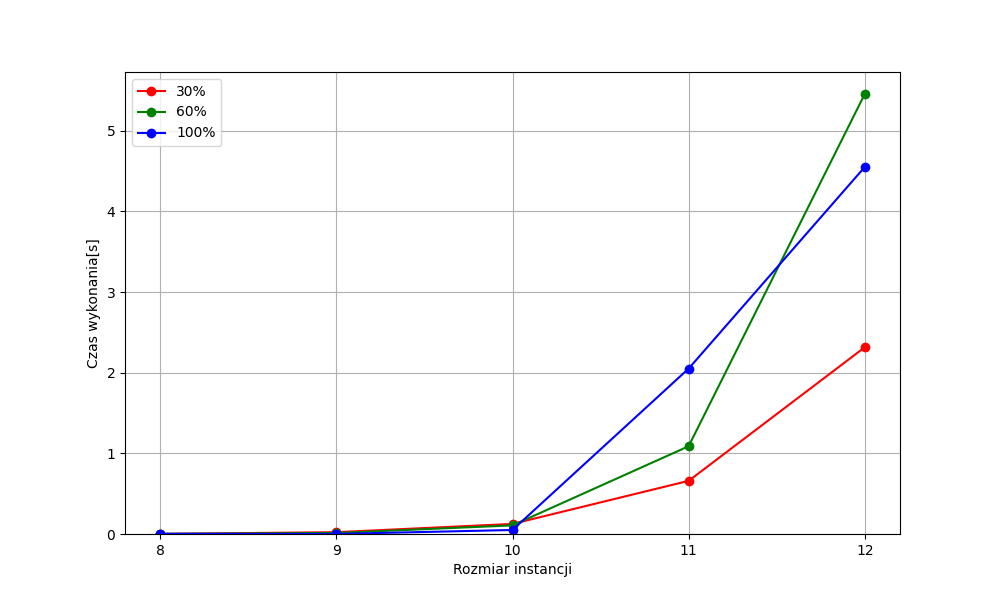
\includegraphics[width=\textwidth]{src/plots/symbrute-forceresoult.png}
    \caption{Wyniki dla macierzy symetrycznych o różnych gęstościach}
    \label{fig:sm_bf}
  \end{figure}
  \FloatBarrier
  \subsubsection{Wnioski}

  \subsection{Metoda podziału i ograniczeń (ang. Branch and bound)}

  \subsection{Przeszukiwanie w szerz (ang. Breadth first search)}
  Lorem
  \subsubsection{Opis algorytmu}
  \subsubsection{Lista kroków}
  \subsubsection{Założenia badawcze}
  \subsubsection{Wyniki}
  \begin{table}[ht]
\centering
\begin{tabular}{rrrrrrr}
\toprule
 & \multicolumn{3}{c}{Symetryczne} & \multicolumn{3}{c}{Asymetryczne} \\
Rozmiar/Gęstość & 30\% & 60\% & 100\% & 30\% & 60\% & 100\% \\
\midrule
8 & 0.000309 & 0.000893 & 0.021742 & 0.000316 & 0.011754 & 0.027044 \\
9 & 0.001921 & 0.005820 & 0.183279 & 0.002084 & 0.065804 & 0.216008 \\
10 & 0.006027 & 0.036310 & 1.813179 & 0.006508 & 0.469833 & 1.932505 \\
11 & 0.000742 & 0.227200 & 19.783483 & 0.042772 & 7.037906 & 20.387592 \\
12 & 0.003750 & 1.682285 & 239.443230 & 0.295299 & 25.024631 & 239.564080 \\
\bottomrule
\end{tabular}
\caption{Czasy wykonania algorytmu dla macierzy symetrycznych i niesymetrycznych}
\label{tab:mean_time_bfsresoult}
\end{table}
\begin{table}[ht]
\centering
\begin{tabular}{rrrrrrr}
\toprule
 & \multicolumn{3}{c}{Symetryczne} & \multicolumn{3}{c}{Asymetryczne} \\
Rozmiar/Gęstość & 30\% & 60\% & 100\% & 30\% & 60\% & 100\% \\
\midrule
8 & 30867 & 22264 & 12806 & 28719 & 16340 & 18843 \\
9 & 23923 & 28513 & 7129 & 26942 & 13728 & 17589 \\
10 & 24562 & 39212 & 16436 & 26726 & 14207 & 14841 \\
11 & 40077 & 32101 & 15619 & 39594 & 19117 & 13061 \\
12 & 39712 & 26906 & 17016 & 32837 & 13727 & 12343 \\
\bottomrule
\end{tabular}
\caption{Wyniki algorytmu dla macierzy symetrycznych i niesymetrycznych}
\label{tab:resoult_bfsresoult}
\end{table}
\begin{table}[ht]
\centering
\begin{tabular}{rrrrrrr}
\toprule
 & \multicolumn{3}{c}{Symetryczne} & \multicolumn{3}{c}{Asymetryczne} \\
Rozmiar/Gęstość & 30\% & 60\% & 100\% & 30\% & 60\% & 100\% \\
\midrule
8 & 0.000000 & 0.000000 & 0.000000 & 0.000000 & 0.000000 & 0.090000 \\
9 & 0.000000 & 0.000000 & 0.000000 & 0.000000 & 0.100000 & 0.000000 \\
10 & 0.000000 & 0.000000 & 0.000000 & 0.090000 & 0.150000 & 0.000000 \\
11 & 0.000000 & 0.000000 & 0.000000 & 0.000000 & 0.060000 & 0.040000 \\
12 & 0.000000 & 0.000000 & 0.000000 & 0.000000 & 0.130000 & 0.000000 \\
\bottomrule
\end{tabular}
\caption{Błędy w wynikach algorytmu dla macierzy symetrycznych i niesymetrycznych}
\label{tab:error_bfsresoult}
\end{table}

  \FloatBarrier

  \begin{figure}[ht]
    \centering
    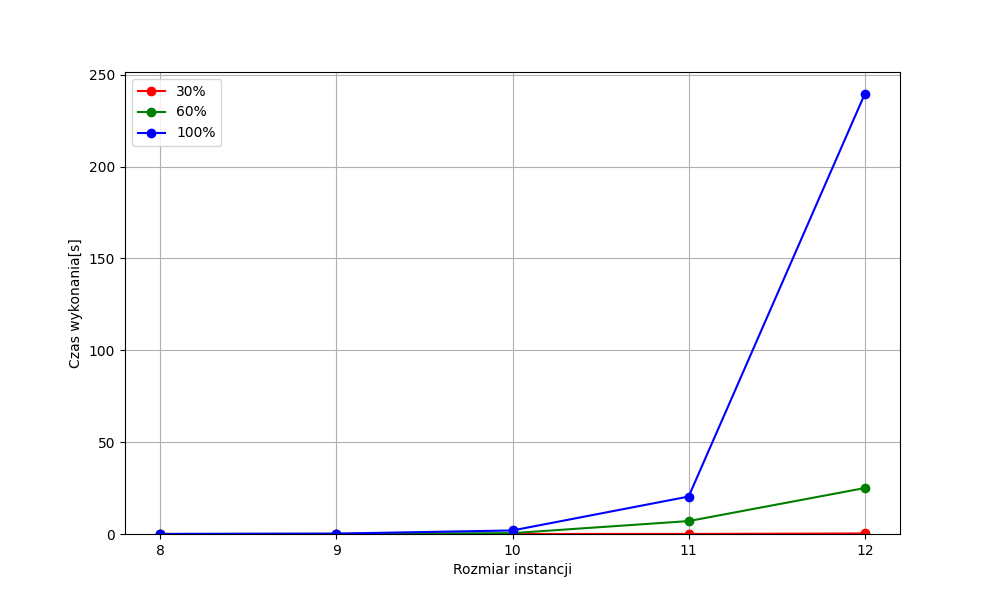
\includegraphics[width=\textwidth]{src/plots/asymbfsresoult.png}
    \caption{Wyniki dla macierzy asymetrycznych o różnych gęstościach}
    \label{fig:asm_bfs}
  \end{figure}    
  \begin{figure}[ht]
    \centering
    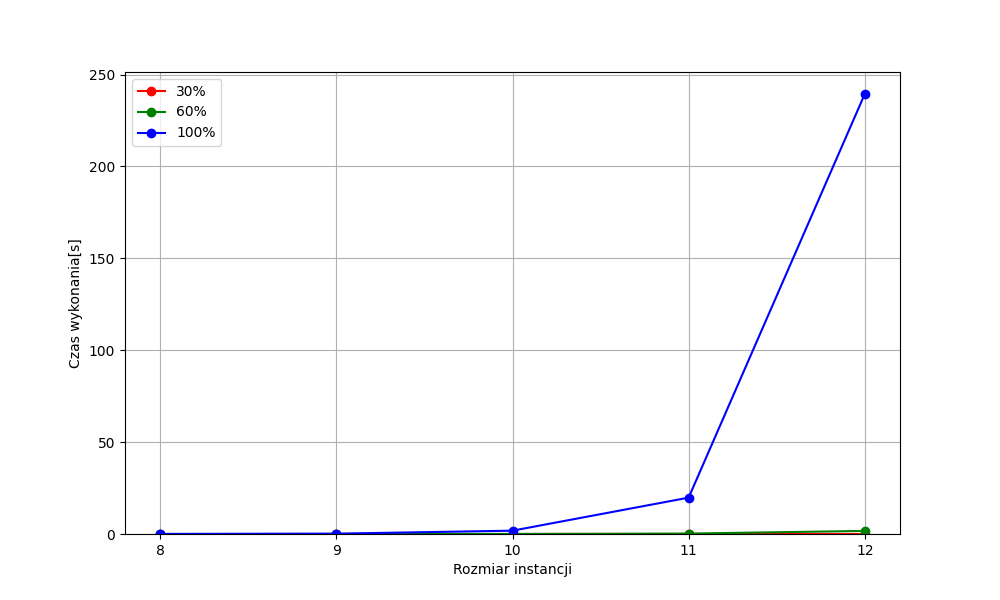
\includegraphics[width=\textwidth]{src/plots/symbfsresoult.png}
    \caption{Wyniki dla macierzy symetrycznych o różnych gęstościach}
    \label{fig:sm_bfs}
  \end{figure}
  \FloatBarrier
  \subsubsection{Wnioski}

  \subsection{Przeszukiwanie w głąb (ang. Depth first search)}
  Lorem
  \subsubsection{Opis algorytmu}
  \subsubsection{Lista kroków}
  \subsubsection{Założenia badawcze}
  \subsubsection{Wyniki}
  \begin{table}[ht]
\centering
\begin{tabular}{rrrrrrr}
\toprule
 & \multicolumn{3}{c}{Symetryczne} & \multicolumn{3}{c}{Asymetryczne} \\
Rozmiar/Gęstość & 30\% & 60\% & 100\% & 30\% & 60\% & 100\% \\
\midrule
8 & 0.000186 & 0.000265 & 0.000635 & 0.000166 & 0.000288 & 0.000634 \\
9 & 0.000363 & 0.000598 & 0.000830 & 0.000751 & 0.000880 & 0.000655 \\
10 & 0.000106 & 0.002801 & 0.004232 & 0.000523 & 0.000546 & 0.004860 \\
11 & 0.000469 & 0.007211 & 0.020066 & 0.012145 & 0.003791 & 0.024452 \\
12 & 0.000246 & 0.007022 & 0.025140 & 0.034566 & 0.015293 & 0.020256 \\
\bottomrule
\end{tabular}
\caption{Czasy wykonania algorytmu dla macierzy symetrycznych i niesymetrycznych}
\label{tab:mean_time_dfsresoult}
\end{table}
\begin{table}[ht]
\centering
\begin{tabular}{rrrrrrr}
\toprule
 & \multicolumn{3}{c}{Symetryczne} & \multicolumn{3}{c}{Asymetryczne} \\
Rozmiar/Gęstość & 30\% & 60\% & 100\% & 30\% & 60\% & 100\% \\
\midrule
8 & 29723 & 22264 & 12806 & 28719 & 14466 & 20755 \\
9 & 23923 & 28513 & 7129 & 26942 & 15282 & 17589 \\
10 & 24562 & 39212 & 16436 & 26830 & 16789 & 14841 \\
11 & 40077 & 32101 & 15619 & 35395 & 20388 & 13657 \\
12 & 39712 & 26906 & 17016 & 32837 & 15782 & 11779 \\
\bottomrule
\end{tabular}
\caption{Wyniki algorytmu dla macierzy symetrycznych i niesymetrycznych}
\label{tab:resoult_dfsresoult}
\end{table}
\begin{table}[ht]
\centering
\begin{tabular}{rrrrrrr}
\toprule
 & \multicolumn{3}{c}{Symetryczne} & \multicolumn{3}{c}{Asymetryczne} \\
Rozmiar/Gęstość & 30\% & 60\% & 100\% & 30\% & 60\% & 100\% \\
\midrule
8 & 0.040000 & 0.000000 & 0.000000 & 0.000000 & 0.110000 & 0.000000 \\
9 & 0.000000 & 0.000000 & 0.000000 & 0.000000 & 0.000000 & 0.000000 \\
10 & 0.000000 & 0.000000 & 0.000000 & 0.080000 & 0.000000 & 0.000000 \\
11 & 0.000000 & 0.000000 & 0.000000 & 0.110000 & 0.000000 & 0.000000 \\
12 & 0.000000 & 0.000000 & 0.000000 & 0.000000 & 0.000000 & 0.050000 \\
\bottomrule
\end{tabular}
\caption{Błędy w wynikach algorytmu dla macierzy symetrycznych i niesymetrycznych}
\label{tab:error_dfsresoult}
\end{table}

  \FloatBarrier

  \begin{figure}[ht]
    \centering
    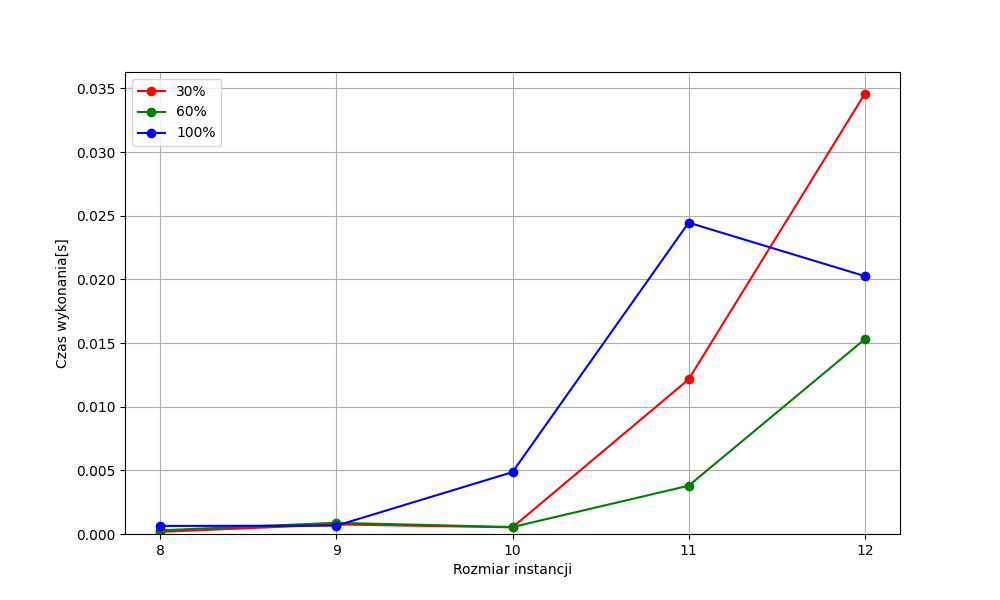
\includegraphics[width=\textwidth]{src/plots/asymdfsresoult.png}
    \caption{Wyniki dla macierzy asymetrycznych o różnych gęstościach}
    \label{fig:asm_df}
  \end{figure}
  \begin{figure}[ht]
    \centering
    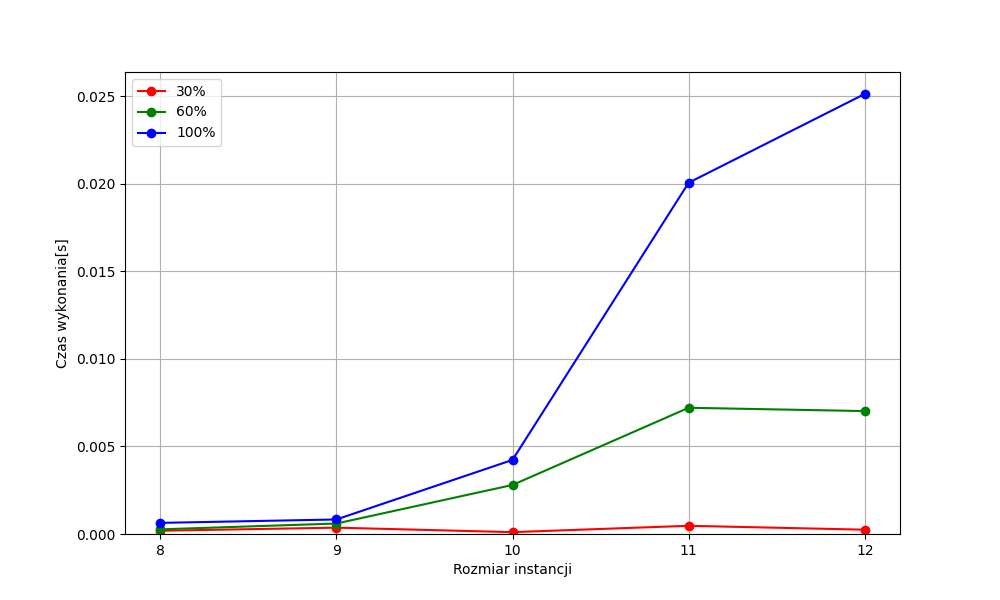
\includegraphics[width=\textwidth]{src/plots/symdfsresoult.png}
    \caption{Wyniki dla macierzy symetrycznych o różnych gęstościach}
    \label{fig:sm_df}
  \end{figure}
  \FloatBarrier
  \subsubsection{Wnioski}

  \subsection{Przeszukiwanie przy minimum kosztów (ang. Least cost)}
  Lorem
  \subsubsection{Opis algorytmu}
  \subsubsection{Lista kroków}
  \subsubsection{Założenia badawcze}
  \subsubsection{Wyniki}
  \begin{table}[ht]
\centering
\begin{tabular}{rrrrrrr}
\toprule
 & \multicolumn{3}{c}{Symetryczne} & \multicolumn{3}{c}{Asymetryczne} \\
Rozmiar/Gęstość & 30\% & 60\% & 100\% & 30\% & 60\% & 100\% \\
\midrule
8 & 0.000182 & 0.000130 & 0.000262 & 0.000268 & 0.000081 & 0.000387 \\
9 & 0.000557 & 0.000336 & 0.000447 & 0.000148 & 0.000803 & 0.001481 \\
10 & 0.000469 & 0.001513 & 0.003302 & 0.001321 & 0.001555 & 0.002506 \\
11 & 0.000641 & 0.009767 & 0.011304 & 0.009657 & 0.002796 & 0.008128 \\
12 & 0.003151 & 0.010295 & 0.016628 & 0.009071 & 0.003136 & 0.002091 \\
\bottomrule
\end{tabular}
\caption{Czasy wykonania algorytmu dla macierzy symetrycznych i niesymetrycznych}
\label{tab:mean_time_leastCostresoult}
\end{table}
\begin{table}[ht]
\centering
\begin{tabular}{rrrrrrr}
\toprule
 & \multicolumn{3}{c}{Symetryczne} & \multicolumn{3}{c}{Asymetryczne} \\
Rozmiar/Gęstość & 30\% & 60\% & 100\% & 30\% & 60\% & 100\% \\
\midrule
8 & 30867 & 22264 & 12806 & 28719 & 16340 & 20755 \\
9 & 23923 & 28513 & 7129 & 26942 & 15282 & 17589 \\
10 & 24562 & 39212 & 16436 & 29310 & 16789 & 14841 \\
11 & 40077 & 32101 & 15619 & 39594 & 20388 & 13657 \\
12 & 39712 & 26906 & 17016 & 32837 & 15782 & 12343 \\
\bottomrule
\end{tabular}
\caption{Wyniki algorytmu dla macierzy symetrycznych i niesymetrycznych}
\label{tab:resoult_leastCostresoult}
\end{table}
\begin{table}[ht]
\centering
\begin{tabular}{rrrrrrr}
\toprule
 & \multicolumn{3}{c}{Symetryczne} & \multicolumn{3}{c}{Asymetryczne} \\
Rozmiar/Gęstość & 30\% & 60\% & 100\% & 30\% & 60\% & 100\% \\
\midrule
8 & 0.000000 & 0.000000 & 0.000000 & 0.000000 & 0.000000 & 0.000000 \\
9 & 0.000000 & 0.000000 & 0.000000 & 0.000000 & 0.000000 & 0.000000 \\
10 & 0.000000 & 0.000000 & 0.000000 & 0.000000 & 0.000000 & 0.000000 \\
11 & 0.000000 & 0.000000 & 0.000000 & 0.000000 & 0.000000 & 0.000000 \\
12 & 0.000000 & 0.000000 & 0.000000 & 0.000000 & 0.000000 & 0.000000 \\
\bottomrule
\end{tabular}
\caption{Błędy w wynikach algorytmu dla macierzy symetrycznych i niesymetrycznych}
\label{tab:error_leastCostresoult}
\end{table}

  \FloatBarrier
  
  \begin{figure}[ht]
    \centering
    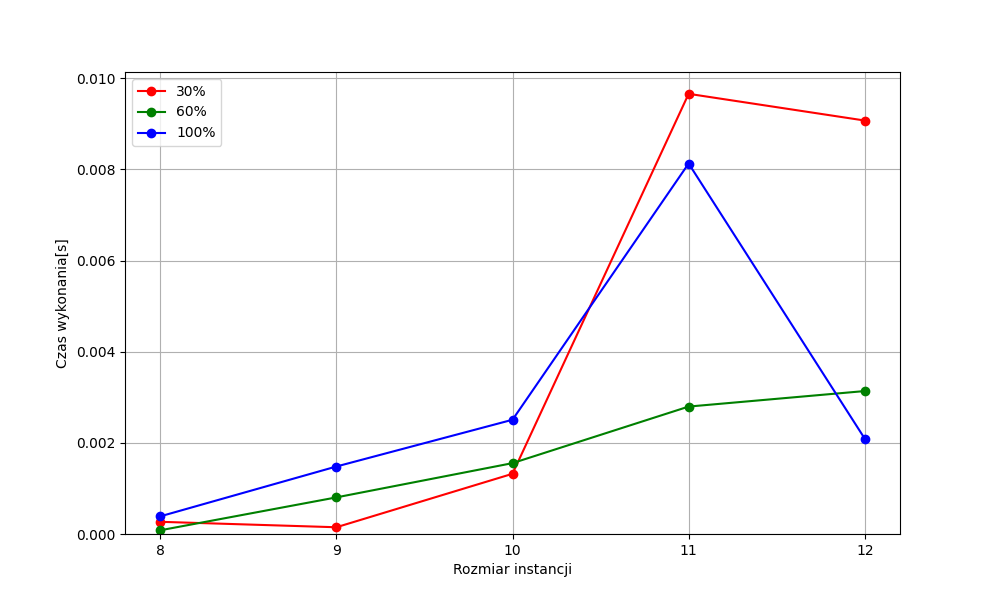
\includegraphics[width=\textwidth]{src/plots/asymleastCostresoult.png}
    \caption{Wyniki dla macierzy symetrycznych o różnych gęstościach}
    \label{fig:asm_lc}
  \end{figure}
  \begin{figure}[ht]
    \centering
    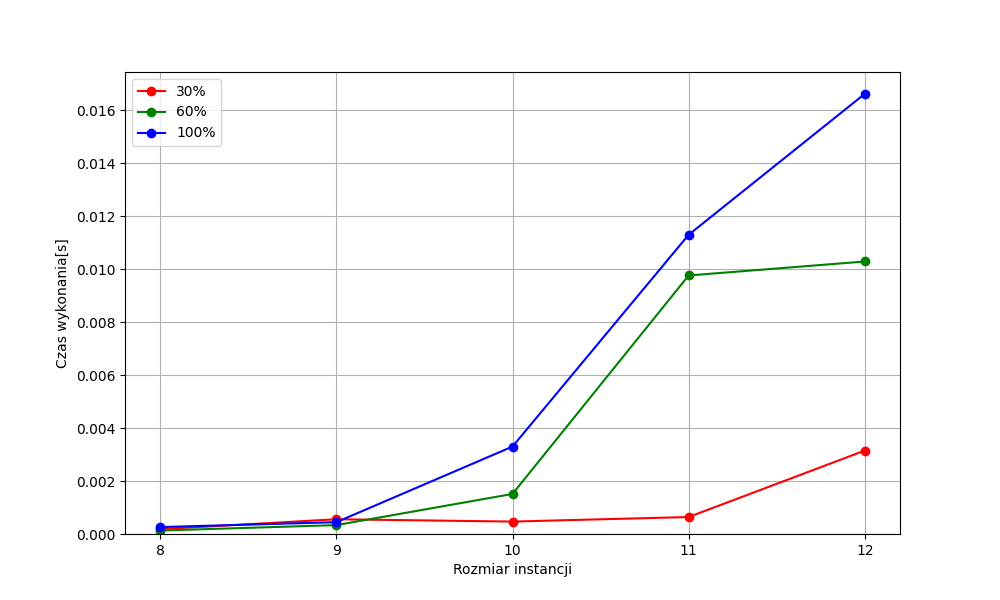
\includegraphics[width=\textwidth]{src/plots/symleastCostresoult.png}
    \caption{Wyniki dla macierzy symetrycznych o różnych gęstościach}
    \label{fig:sm_lc}
  \end{figure}
  \FloatBarrier
  \subsubsection{Wnioski}
  
  \section{Źródła}
  Lorem  ipsum  dolor  sit  amet,  consectetuer  adipiscing  
  elit.   Etiam  lobortisfacilisis sem.  Nullam nec mi et 
  neque pharetra sollicitudin.  Praesent imperdietmi nec ante. 
  Donec ullamcorper, felis non sodales...
\end{document}